
%%\subsection{The Basic Problem That We Studied}

\begin{frame}
  \frametitle{What I hope you take away from this talk}
  \begin{itemize}
  \item A broad outline of multiple scattering theory with enough
    background to talk with a theorist
  \item An understanding of how multiple scattering theory is used to
    interpret \textbf{XANES} spectra
  \item An understanding of how multiple scattering theory is used to
    analyze \textbf{EXAFS} spectra
  \item Some ideas about how to incorporate multiple scattering theory
    in your research
  \end{itemize}
\end{frame}

\begin{frame}
  \frametitle{This talk is about Feff}

  There are many approaches to spectroscopy theory out there,
  including multiplets, band structure, and finite difference methods.

  \bigskip

  \begin{exampleblock}{This talk is about Feff}
    \begin{center}
      \textsc{feff} is a real-space, multiple scattering code.
    \end{center}
  \end{exampleblock}
  
  \bigskip

  \begin{itemize}
  \item A conceptual summary and simple physical interpretation of
    what ``real-space multiple scattering'' means.
  \item How RSMS is used to make XANES calculations.
  \item How RSMS is used in fitting EXAFS data.
  \end{itemize}

\end{frame}

\begin{frame}
  \frametitle<1| handout:1>{A simple picture of X-ray absorption} 
  \frametitle<2| handout:2>{X-ray absorption in condensed matter}

  \begin{overlayarea}{\linewidth}{6ex}
    \only<1| handout:1>{An incident x-ray of energy $E$ is absorbed,
      destroying a core electron of binding energy $E_0$ and emitting
      a photo-electron with kinetic energy $(E-E_0)$. The core state
      is eventually filled, ejecting a fluorescent x-ray or an Auger
      electron.  }%
    \only<2| handout:2>{The ejected photo-electron can scatter from
      neighboring atoms. $R$ has some relationship to $\lambda$ and
      there is a phase shift associated with the scattering event.
      Thus the outgoing and scattered waves interfere.  }%
  \end{overlayarea}

  \vskip 20pt

  \begin{columns}[T]
    \begin{column}{0.5\linewidth}
      \only<1| handout:1>{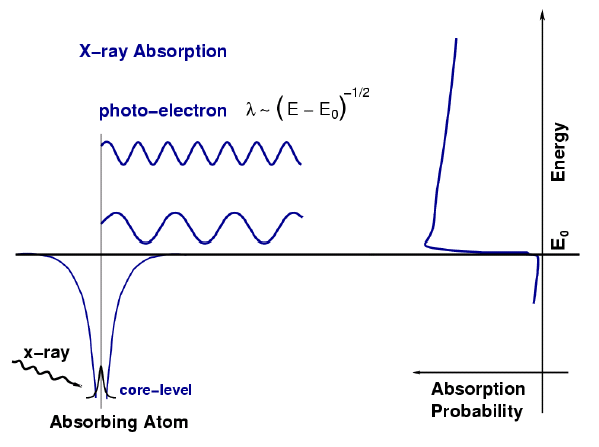
\includegraphics[width=\linewidth]{bare_atom.png}}
      \only<2| handout:2>{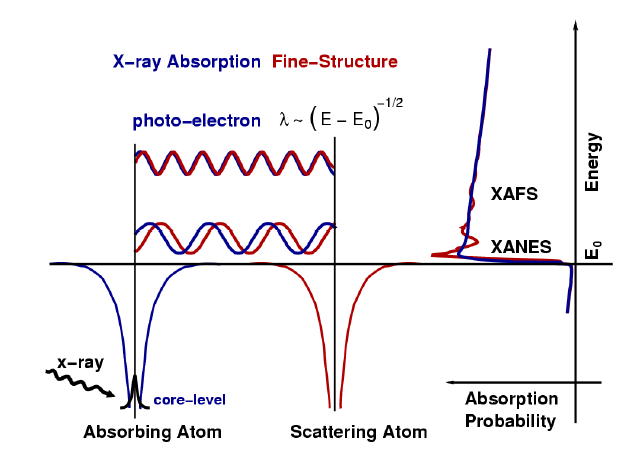
\includegraphics[width=\linewidth]{with_scattering.png}}
    \end{column}
    \begin{column}{0.5\linewidth}
      \begin{center}
        \only<1| handout:1>{
          An empty final state is required.\\
          {\alert{No available state, \\
              no absorption!}}\\
          When the incident x-ray energy is larger than the binding
          energy, there is a sharp increase in absorption.
        }
        \only<2| handout:2>{
          The scattering of the photo-electron wave function interferes
          with itself.\\[4ex]
          $\mu(E)$ depends on the density of states with energy
          $(E-E_0)$ at the absorbing atom.
        }
      \end{center}
    \end{column}
  \end{columns}

  \vskip 20pt

  \begin{overlayarea}{\linewidth}{3ex}
    \only<1| handout:1>{For an isolated atom, $\mu(E)$ has a sharp step at the
      core-level binding energy and is a smooth function of energy
      above the edge.}%
    \only<2| handout:2>{This interference \alert{at the absorbing atom} will vary
      with energy, causing the oscillations in $\mu(E)$.
    }%
  \end{overlayarea}
  \begin{bottomnote}[0.7][20] 
    Image from Matt Newville
  \end{bottomnote}
\end{frame}


\begin{frame}
  \frametitle{Computing X-ray Absorption from First Principles}
  \begin{columns}
    \begin{column}{0.75\linewidth}
      In XAS we measure the \emph{dipole mediated}$^\mathrm{[1]}$ transition of
      an electron in a \emph{deep core}$^\mathrm{[2]}$ state
      {\color{blue}$|i\rangle$} into an \emph{unoccupied}$^\mathrm{[3]}$ state
      {\color{red}$|f\rangle$}:


      \begin{block}{Fermi's Golden Rule}
        \centering
        $\mu(E) \propto\> \sum\limits_f^{E_f>E_F}
        \big|{\color{red}\langle f|}
        {\color{blue}\hat{\epsilon}\cdot\mathbf{r}}
        {\color{blue}|i\rangle}\big|^2
        \delta(E_f)$
      \end{block}

      Broadly speaking, there are two ways to solve this equation:
      \begin{enumerate}
      \item Accurately represent {\color{blue}$|i\rangle$}$^\mathrm{[4]}$  and
        {\color{red}$|f\rangle$}$^\mathrm{[5]}$, then evaluate
        the integral directly. This is the approach taken, for example, by
        molecular orbital theory.
      \item Use multiple scattering theory, AKA a Green's
        function$^\mathrm{[6]}$ or propagator formalism:\\
        {\footnotesize
        $\mu(E) \propto
        -\frac{1}{\pi} \Im {\color{blue}\langle \mathrm{i}
          |} \hat{\epsilon}^\ast \cdot \boldsymbol{r} \,
        {\color{Green4}\mathbb{G}(r,r';E)} \hat{\epsilon} \cdot \boldsymbol{r}' {\color{blue}|
          \mathrm{i} \rangle}
        \Theta(E-E_F)$.}
      \end{enumerate}      
    \end{column}
    \begin{column}{0.25\linewidth}
      \begin{enumerate}
      \tiny
      \item A photon interacts with an electron
      \item Typically a \textit{1s}, \textit{2s}, or \textit{2p} electron
      \item A bound or continuum state \textbf{not} already containing
        an electron
      \item Easy, basic Q.M.
      \item Hard work, lots of computation
      \item {\color{Green4}$\GMS$} is called a Green's function.
    \end{column}
  \end{columns}
\end{frame}

\begin{frame}
  \frametitle{Real Space Multiple Scattering}

  In multiple scattering theory, all the hard work is in computing
  the Green's function.

  \begin{description}
  \item[${\color{Green4}\GMS}$] the function that describes all
    possible ways for a photoelectron to interact with the
    surrounding atoms
  \item[$\Gnot$] the function that describes how an electron
    propagates between two points in space
  \item[$\tmat$] the function that describes how a photo-electron
    scatters from a neighboring atom
  \end{description}

  \begin{block}{Expanding the Green's function}
    \begin{align}
      {\color{Green4}\GMS} =& \big(1 - \Gnot \tmat\big)^{-1} \, \Gnot \tag{XANES}\\
      =& \Gnot + \Gnot\,\tmat\,\Gnot +
      \Gnot\,\tmat\,\Gnot\,\tmat\,\Gnot +
      \Gnot\,\tmat\,\Gnot\,\tmat\,\Gnot\,\tmat\,\Gnot + ... \tag{EXAFS}
    \end{align}
  \end{block}
\end{frame}

\begin{frame}{Scattering Paths}
  Solving {\color{DarkOrchid4} ${\color{Green4}\GMS} = \big(1 - \Gnot
    \tmat\big)^{-1} \, \Gnot$} considers these and {\LARGE ALL} other
  paths within some cluster of atoms:

  \begin{tabular}[t]{ccc}
    {\color{DarkOrchid4}single scattering path} & {\color{blue}\SS} & (2 legs)\\
    {\color{DarkOrchid4}double scattering path} & \includegraphics[width=0.2\linewidth]{images/ds}& (3 legs)\\
    {\color{DarkOrchid4}triple scattering path} & \includegraphics[width=0.2\linewidth]{images/ts}& (4 legs)\\
  \end{tabular}

  \medskip

  \begin{center}
    The clever thing about \textsc{feff} is that each term is further
    expanded as a sum of all paths of that order.

    {\color{DarkOrchid4}$\Gnot\,\tmat\,\Gnot$} is expanded as a sum of
    {\color{DarkOrchid4}single scattering} paths

    {\color{DarkOrchid4}$\Gnot\,\tmat\,\Gnot\,\tmat\,\Gnot$} is a sum
    of all {\color{DarkOrchid4}double scattering} paths

    and so on.
  \end{center}

\end{frame}

%%% Local Variables:
%%% mode: latex
%%% TeX-master: t
%%% End:
